\documentclass{assignment}

\usepackage{float}
\usepackage{tikz}
\usepackage{adjustbox}
\usepackage{titlesec}
\usepackage{soul}
\usepackage{csvsimple}

\usepackage{graphicx}
\usepackage{subcaption}
\usetikzlibrary{shapes, arrows}

\usepackage{bm}
\usepackage{amsmath,amssymb}

\usetikzlibrary{calc,patterns,angles,quotes}
\setlength{\parindent}{0pt}

\hypersetup{
pdftitle={Topology Optimisation},
pdfsubject={Structural optimisation of a truss structure},
pdfauthor={Tommaso Bocchietti}
}

\makeglossaries

\begin{document}

\title{Topology Optimisation \\ Structural optimisation of a truss structure}
\author{Tommaso Bocchietti 10740309}
\date{A.Y. 2024/25}

\maketitle

\begin{figure}[H]
    \centering
    
\includegraphics[width=0.7\textwidth]{./pdf/Polimi_logo_coverpage.pdf}
    \label{fig:Polimi_logo}
\end{figure}

\clearpage
\tableofcontents
\listoffigures
\listoftables
\lstlistoflistings
% \printglossary[type=\acronymtype]

\clearpage
\section{Requests}
\label{sec:requests}

The goal of this project is to perform a topology optimisation of a truss structure, minimising the compliance $C$ of the structure subjected to a volume constraint $V - V_0 \le 0$.

The structure is a 2D truss with a fixed geometry and a fixed load as shown in Figure \ref{fig:truss}.

\begin{figure}[H]
    \centering
    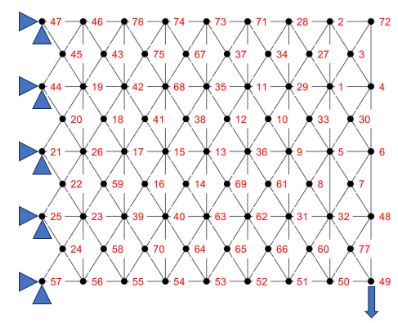
\includegraphics[width=0.7\textwidth]{img/structure.png}
    \caption{Truss structure}
    \label{fig:truss}
\end{figure}

We can summarise the given data as follows:

% \begin{table}
%     \centering
%     \begin{tabular}{|c|c|}
%         \hline
%         \textbf{Parameter} & \textbf{Value} \\
%         \hline
%         $E$ & $1 \times 10^7$ N/m$^2$ \\
%         $A$ & 0.01 m$^2$ \\
%         $V_0$ & 0.1 m$^3$ \\
%         $P$ & 1000 N \\
%         \hline
%     \end{tabular}
%     \caption{Given data}
%     \label{tab:given_data}
% \end{table}


The formal definition of the request is to perform a topology optimisation for the four cases presented in Table \ref{tab:cases}.

\begin{table}[H]
    \centering
    \begin{tabular}{|c|c|c|c|}
        \hline
        \textbf{Case} & \textbf{$\alpha$} & \textbf{Lower bound $[mm^2]$} & \textbf{Upper bound $[mm^2]$} \\
        \hline
        1             & 0.05              & 0.0001                        & 800                           \\
        2             & 0.10              & 0.0001                        & 800                           \\
        3             & 0.15              & 0.0001                        & 800                           \\
        4             & 0.20              & 0.0001                        & 800                           \\
        \hline
    \end{tabular}
    \caption{Optimisation cases}
    \label{tab:cases}
\end{table}

Here, the parameter $\alpha$ is the volume fraction of the structure, defined as $\alpha = \frac{V_0}{V_{max}}$, where $V_{max} = UB \sum_{j=1}^{N_{beams}} l_j$ is the maximum volume of the structure.
\section{Methodology}
\label{sec:methodology}

Before starting the optimisation process, we need to define the problem in mathematical terms.
The goal of the project is to minimise the compliance $C$ of the structure subjected to a volume constraint $V - V_0 \le 0$.

In the following sections, we will give an overview of the equations and the theroetical background needed to solve the problem.
We will then move on to the implementation of the optimisation algorithm and the results obtained.
\section{Theoretical background}
\label{sec:theoretical_background}

\subsection{General topology optimisation problem}
\label{subsec:general_topology_optimisation_problem}

Topology optimisation is a mathematical method that optimises the material distribution within a given design domain to achieve the best performance of a structure.
The goal is to find the optimal distribution of material that minimises a certain objective function, subject to a set of constraints.

The general topology optimisation problem can be formulated as follows:
\begin{equation}
    \begin{aligned}
         & \underset{x}{\text{minimise}} &  & f(\bm{u}, \bm{u}_0, \bm{x})       \\
         & \text{subject to}             &  & g(\bm{u}, \bm{u}_0, \bm{x}) \le 0 \\
         &                               &  & h(\bm{u}, \bm{u}_0, \bm{x}) = 0   \\
         &                               &  & \bm{x} \in \Omega
    \end{aligned}
    \label{eq:general_topology_optimisation_problem}
\end{equation}

where:

\begin{itemize}
    \item $\bm{x}$ is the design variable, representing the material distribution within the design domain $\Omega$.
    \item $\bm{u}$ is the displacement field.
    \item $\bm{u}_0$ is the displacement field of the reference structure.
    \item $f(\bm{u}, \bm{u}_0, \bm{x})$ is the objective function, representing the performance of the structure.
    \item $g(\bm{u}, \bm{u}_0, \bm{x})$ is the inequality constraint function.
    \item $h(\bm{u}, \bm{u}_0, \bm{x})$ is the equality constraint function.
    \item $\Omega$ is the design domain.
\end{itemize}

The design variable $\bm{x}$ is a vector of size $n$, where $n$ is the number of elements in the design domain.
Each element $x_i$ of the design variable $\bm{x}$ represents the material density of the corresponding element in the design domain.
The material density $x_i$ is a scalar value between 0 and 1, where 0 represents void (no material) and 1 represents solid material.

The objective function $f(\bm{u}, \bm{u}_0, \bm{x})$ is a measure of the performance of the structure, such as compliance, mass, or stress.

The inequality constraint function $g(\bm{u}, \bm{u}_0, \bm{x})$ represents the physical constraints of the problem, such as volume constraints, stress constraints, or displacement constraints.

As we will see in the next sections, the general topology optimisation problem can be tailored to specific applications with different objective functions and constraints.
In the following, the most important ones will be presented.


\subsubsection{Compliance minimisation problem}
\label{subsubsec:compliance_minimisation_problem}

The compliance minimisation problem is one of the most common topology optimisation problems.

Compliance is a measure of the flexibility of a structure under a given load.
It is defined as the work done by the external forces to deform the structure by a certain amount.
The compliance $C$ of a structure can be calculated as follows:

\begin{equation}
    C = \bm{F}^T \bm{u}
    \label{eq:compliance}
\end{equation}

where $\bm{F}$ is the vector of external forces applied to the structure and $\bm{u}$ is the displacement field of the structure.

In many cases, the compliance minimisation problem is subject to a volume constraint, which limits the amount of material that can be used in the design.
The volume constraint can be formulated as follows:

\begin{equation}
    V - V_0 \le 0
    \label{eq:volume_constraint}
\end{equation}

where $V$ is the volume of the structure and $V_0$ is the target volume of the structure.

The compliance minimisation problem with a volume constraint can be formulated as follows:

\begin{equation}
    \begin{aligned}
         & \underset{\bm{x}}{\text{minimise}} &  & C(\bm{u}, \bm{F}, \bm{x}) \\
         & \text{subject to}                  &  & V(\bm{x}) - V_0 \le 0     \\
         &                                    &  & \bm{x} \in [0, 1]^n
    \end{aligned}
    \label{eq:compliance_minimisation_problem}
\end{equation}


\subsubsection{Volume minimisation problem}
\label{subsubsec:volume_minimisation_problem}

The volume minimisation problem is another common topology optimisation problem.

The goal of the volume minimisation problem is to find the minimum amount of material required to support a given load.
This problem is often used in the design of lightweight structures, where the goal is to reduce the weight of the structure while maintaining its structural integrity.

The volume minimisation problem can be formulated as follows:

\begin{equation}
    \begin{aligned}
         & \underset{\bm{x}}{\text{minimise}} &  & V(\bm{x})                         \\
         & \text{subject to}                  &  & C(\bm{u}, \bm{F}, \bm{x}) \le C_0 \\
         &                                    &  & \bm{x} \in [0, 1]^n
    \end{aligned}
    \label{eq:volume_minimisation_problem}
\end{equation}

where $V(\bm{x})$ is the volume of the structure, $C(\bm{u}, \bm{F}, \bm{x})$ is the compliance of the structure, and $C_0$ is the target compliance of the structure.


\subsection{Mathematical foundation}
\label{subsec:mathematical_foundation}

Topology optimisation is based on the mathematical theory of optimisation, which deals with finding the best solution to a given problem.

As we already know form calculus, the optimal solution to a given problem can be found in correspondence of the minimum or maximum of a function.
Of course, minimun and maximum can be found by looking at the first and second derivative of the function.

When dealing with topology optimisation, the objective function $f(\bm{u}, \bm{u}_0, \bm{x})$ is usually non-linear multi-variable function, which makes the optimisation problem more complex.

In order to solve the topology optimisation problem, numerical optimisation algorithms are used.
These algorithms are designed to find the optimal solution to a given problem by iteratively updating the design variable $\bm{x}$ until the objective function is minimised or maximised.

The most common optimisation algorithms used in topology optimisation are gradient-based algorithms, such as the method of steepest descent, the conjugate gradient method, and the quasi-Newton method.
These algorithms use the gradient of the objective function to update the design variable $\bm{x}$ in each iteration.

In the next sections, we will see how these optimisation algorithms can be applied to solve the compliance minimisation problem and the volume minimisation problem.






% \clearpage
% \bibliographystyle{plain}
% \bibliography{ref}

\end{document}
